\chapter{Calibration Strategy}
\label{ch:exec-summ-calib}

%%%%%%%%%%%%%%%%%%%%%%%%%%%%%%%%%%%%%%%%%%%%%%%%%%%%%%%%%%%%%%%%%%%%
\section{Introduction}
\label{sec:calibintro} %% 2 pages


The DUNE \dword{fd} presents a unique challenge for calibration in many ways. Not only because of its size---the largest \dword{lartpc} ever constructed -- but also because of its depth. It differs both from existing long-baseline neutrino detectors, and existing \dwords{lartpc}. Also, the deep underground location results in low cosmic ray rates limiting the usage of it as a calibration source. Another important difference is that DUNE does not as yet have a near detector design and, unlike MINOS and \dword{nova}, the near detector is unlikely to be very much like the \dword{fd}.

Like any \dword{lartpc}, DUNE has as a great advantage precision tracking and ultra-clean target medium, but, to fully exploit this will require significant challenges in understanding its detector response. This challenge is driven by the inherently highly convolved detector response model and strong correlations that exist between various calibration quantities. For example, the
drift vertex of a track, the drift distance, the initial time the track occurs ($t_0$) and the drift velocity are all highly correlated. In turn, the drift velocity depends on the electric field. The electric field itself may have local variations in space or in time for an enormous detector operating for multiple decades.
The determination of energy associated to an event of interest will depend on the simulation model, associated parameters, non-trivial correlations between the parameters and spatial and temporal dependence of those parameters. A convincing measurement of CP violation, or a resolution of the neutrino mass ordering, will require a demonstration that the overall detector response is well understood, and can be extrapolated across the entire physics regions of interest.

This document will describe a strategy for detector calibration for both 
\dwords{spmod} and \dwords{dpmod}
using dedicated  \dword{fd} systems and/or existing calibration sources. A large portion of the calibration work reported here is done under the joint  \dword{sp} and \dword{dp} Calibration task force (TF) group formed in Fall 2017. Calibration sources and systems provide measurements of the detector response model parameters, or provide tests of the response model.
Figure~\ref{fig:calibneeds} shows the broad range of categories of measurements calibrations can provide. In addition to this, calibration measurements also provide corrections applied to data, data-driven efficiencies, systematics and particle responses. Figure~\ref{fig:calibneeds} also lists some of the critical calibration parameters for DUNE's detector response model for either  \dword{sp} or \dword{dp}.
Due to the significant interdependencies of many parameters (recombination, drift velocity, electric field), a calibration strategy will either need to iteratively measure parameters, and/or find sources which break these correlations. 

\begin{dunefigure}[Categories of measurements provided by Calibration.]{fig:calibneeds}{Categories of measurements provided by Calibration.}
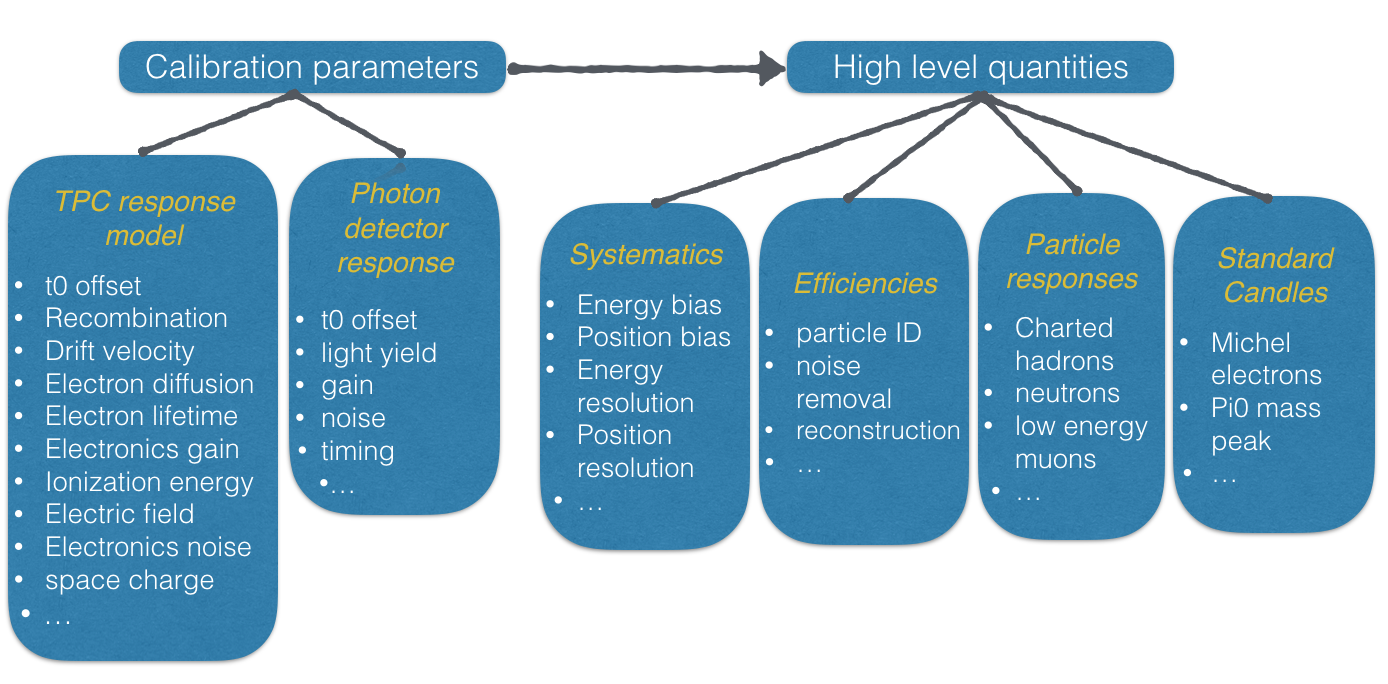
\includegraphics[width=.9\textwidth]{calib-needs.png}
\end{dunefigure}

The systematic uncertainties on high level physics quantities drive how precisely each parameter need to be measured. For example, how precisely will the drift velocity need to be measured to know fiducial volume better than \num{1}\%?  What does \num{1}\% energy bias mean for electron drift-lifetime and electronics calibration measurements? Section~\ref{sec:calibphys} describes the physics requirements for calibration for long-baseline, supernovae and other physics such as nucleon decay and exotic searches. In general, the calibration program must provide measurements at the few percent or better level, and must also provide sufficient redundancy in the measurement program.

Section~\ref{sec:existsource} describes existing calibration sources, their limitations and remaining studies necessary for the TDR. Existing calibration sources include (beam or atmospheric)  neutrino-induced samples, cosmic rays, argon isotopes and instrumentation devices such as liquid argon purity monitors, temperature and current monitors. For example, drift velocity depends on  temperature (and electric field), so measurements of temperature reduce the interdependencies in understanding drift velocity. While there are many existing calibration sources, each source comes with its own challenges. We further distinguish between sources which are used to measure a response model parameter, and measurements which test the response model. For example, electrons from pion or muon decay (Michel electrons) are very useful to study the detector response to low energy electrons ($\sim$ \SI{50}{\MeV}). However, low-energy electrons have major reconstruction challenges due to the loss of charge from radiative photons as demonstrated in \dword{microboone}\todo{add DC reference}. Therefore, Michel electrons are considered as an important, independent, and necessary test of the response model, and not as a measurement of a particular response parameter.

Section~\ref{sec:extcalib} describes calibration measurements from 
other \dword{lar} experiments that are of relevant for DUNE. This includes both past measurements (e.g., ArgoNeuT, DUNE \dword{35t}, \dword{microboone}, LArIAT), anticipated measurements from ongoing and future experiments (e.g., \dword{microboone}, \dword{protodune}) as well as from small scale \dword{lartpc} test stands. Some parameters, like the argon ionization energy, are believed to be universal and have been measured ex-situ. \Dword{protodune} and previous measurements are independent, critical tests of the response model, where the choice of parameterization and values correctly reproduces real detector data. However informative, not all of the previous ex-situ measurements will be directly extrapolatable to DUNE.

Section~\ref{sec:extsystems} describes dedicated external calibration systems currently under consideration for DUNE to perform calibration that cannot be achieved fully from existing sources or external measurements. For each system considered, a reference design is described along with motivation, possible measurements and remaining studies. All the systems proposed are currently being actively discussed and agreed as critical systems by the DUNE collaboration.

Section~\ref{sec:calibsum} provides a summary of the document along with future steps for calibration and a path to TDR.  While the proposed external calibration systems are being finalized, the calibration TF 
focused on finalizing the feedthrough penetration design for the \dword{spmod} and made necessary accommodations for calibration systems. The current cryostat penetration design for \dword{spmod}  calibrations is described in Section~\ref{sec:FTs}. The TF will soon start focusing on \dword{dpmod}  design and accommodations in terms of calibration penetrations. Under current assumptions, the calibration strategy and proposed calibration systems described in this document are applicable to both \dwords{sp} and \dwords{dp}. Any specific differences with \dword{sp} and additional considerations for  \dword{dp}  are interspersed through out the document where necessary. One of the biggest challenges of \dword{dp} is the \SI{12}{\m} long single drift path and ion accumulation at the liquid-gas interface. This is discussed in more detail in Section \todo{add the section}. 
    
%%%%%%%%%%%%%%%%%%%%%%%%%%%%%%%%%%%%%%%%%%%%%%%%%%%%%%%%%%%%%%%%%%%%%%
\section{Physics Requirements for Calibration Systems}
\label{sec:calibphys} %% 3 pages

 DUNE has a broad physics program with needs served by calibration. Section~\ref{sec:lbl} describes the impact of calibration-driven physics on the long baseline program, Section~\ref{sec:sn} describes the supernova physics program which relies on low-energy interactions, and Section~\ref{sec:exotica} describes exotic physics model searches, including nucleon decay. 
 
 Most of the studies done so far are generic, that is they demonstrate the impact of categories of effects. For example, the impact of energy bias is discussed for the long baseline analysis, and such bias can stem from: the neutrino interaction model, insufficient calibration, or reconstruction pathologies. For this note, we take as a target that calibration, by itself, needs to be sufficient for DUNE's program; other issues which limit the physics program are out of scope and errors always add in quadrature. 
 
%%%%%%%%%%%%%%%%%%%%%%%%%%%%%%%%%%%%
\subsection{Long-baseline physics }\label{sec:lbl}
%- Kendall (first pass) and Sowjanya}

DUNE's \dword{lbl} program %long baseline program (LBL) 
uses measurements of % $\nu_e$, $\overline{\nu}_e$ 
\nue, \anue appearance and \numu %$\nu_\mu$ 
disappearance, to probe for new physics with neutrinos, including a search for CP violation (\dword{cpv}), and the mass hierarchy. Additional far detector physics includes measurements with atmospheric neutrinos, $\nu_\tau$ appearance, and non-standard matter  interactions or other effects. These programs all
rely on neutrinos of energies 0.2-10 GeV. 

In the physics volume of the DUNE CDR~\cite{cdr-2}, Figure~3.23 shows that increasing the uncertainties on the \nue event rate from 
\num{2}\% overall\footnote{This uncertainty is an uncorrelated normalization uncertainty on the far detector \nue rate in a four sample FD fit that assumes reasonable near detector constrains on flux and cross sections.} to \num{3}\% results in a \num{50}\% longer run period, 
The CDR also assumes that the fiducial volume is understood at the 1\% level. Thus, calibration information needs to provide approximately 1-2\% understanding of normalization, energy and position resolution within the detector. Studies by E. Worcester
\fixme{do we want names in the text? Anne} in March 2016~\cite{ebias} expanded the simple treatment of energy  presented above. In particular, \num{1}\% bias on the lepton energy has a significant impact on the sensitivity to \dword{cpv}. A \num{3}\% bias in the hadronic state (excluding neutrons), is important as well, as the Bjorken $y$ distribution for neutrinos and antineutrinos are quite different, a larger fraction of the  antineutrino's energy will go into the hadronic state.  Finally, while studies largely consider a single, absolute energy scale, relative spatial differences across the enormous DUNE \dword{fd} volume will need to be monitored and corrected; this is also true for changes which occur in time requiring detection and correction.

The estimate of the calibrated signal received at the anode ($dQ/dx$) depends on\todo{add reference}:

\begin{equation}
dQ/dx = dE/dx \times \frac{1}{W} \times R \times L \times D \times C
\end{equation}
% FOrumula from J. Klein talk at Aug 2017 CM: https://indico.fnal.gov/event/13293/session/12/contribution/90/material/slides/0.pdf

where $dE/dx$ is the energy lost by the initial particle through ionization through a distance $dx$, $W$ is the energy needed to free an electron, $R$ is the recombination of electrons to Ar${^-}$ atoms, $L$ is the lifetime of electrons, $D$ is diffusion, and $C$ is the calibration of electronics response. For a particle not traveling parallel to the wire, $dx = |dy+dz+v_d t|$, where $dy$ and $dz$ are the distances in the $y$ and $z$ directionS, and the $x$ (drift) direction position depends on the drift velocity ($v_d$).

The electric (E) field  has a critical role in the DUNE as the E field impacts drift velocity, recombination, and therefore the energy estimate ($dQ/dx$). Approximately, a \num{1}\% distortion to the E field will correspond to a \num{0.25}\% distortion to $dQ/dx$. Distortions of the E field can occur locally or globally, and are due to a variety of effects. For example, \dword{cpa} misalignment,  \dword{cpa} structural deformations, and APA/CPA offsets  may create E field distortions localized in space. Non-uniform resistivity in the voltage dividers which create the E field may create a net E field distortion localized in space, and a failure of a resistor will create a sudden change in time. Penetrations to the field cage will also create distortions to the E field. Finally, accumulation of slow moving positive ions, created from cosmic rays or from Ar39 localized in space (``space charge'') will distort the E field. Each individual E field distortion sources may add in quadrature with other effects, and can exceed \numrange{1}{4}\,\% overall E field distortion.
We note that if DUNE does not run at nominal E field, then recombination is higher, and the drift time is longer. Both of these effects make   make the understanding of E field in-situ even more important. Distortions to the electric field also create spatial deformations which propagate to $dQ/dx$. Examples of this include space charge, and misalignments. These distortions occur in three dimensions, but the dominant effect is in the drift direction (the direction of the nominal E field, $x$), so for this document, we estimate the scale of these effects only in $x$.

Spatial deformations within the detector  can also impact the energy estimator. Particles in the detector will repeatedly (elastic) Coulomb scatter with the liquid resulting in small, randomized deviations to their path. Multiple Coulomb Scattering (MCS) is used estimate the particles initial energy, but relies on a known distance the particles traveled. If the  distance is different than expectation due to misalignments or E field spatial deformations, then this may bias the estimator. % http://meroli.web.cern.ch/meroli/lecture_multiple_scattering.html
The fiducial volume (and position resolution) is impacted by our understanding of the distances within the detector, drift velocity and electric field. Like the energy scale case, fiducial volume is affected by relative distortions across the detector either from spatial or temporal causes.
%The drift Drift distance -> Drift velocity affects FV via formula. Spatial distortions also affect MCS, FV.

The stringent physics requirements on energy scale and fiducial volume therefore put similarly stringent requirements onto E field, spatial deformations (alignment), drift velocity, electron lifetime, and the time dependences of these quantities.

The remaining studies to clarify the role of calibration planned in conjunction with the long baseline program are:
\begin{itemize}
\item Quantify the distortion (at truth level quantities) on muon, electron, pion, proton tracks from E field distortions, misalignment, and other known effects which calibration probes. The impact should also be assessed for overall calorimetry (below particle tracking or ID threshold). 
\item Quantify the relative importance of electromagnetic shower photons below pair production threshold. %Not sure what the current outlook on this is, but last I heard (4-5 years ago) it would limit electron energy calibration to ~6-7%, even if everything else was perfect.

\end{itemize}

%%%%%%%%%%%%%%%%%%%%%%%%%%%%%%%%%%%%
\subsection{Exotic Physics}\label{sec:exotica}

Nucleon Decay and other exotic physics calibration needs are comparable to the \dword{lbl} program.
 Signal channels for light dark matter and sterile neutrino searches will be neutral current interactions which are background to the \dword{lbl} physics program and so are discussed earlier. \fixme{reference section (Anne)} The nucleon decay group has done studies of detection of the proton decay channel \ptoknubar, %$p\rightarrow K+ \overline{\nu}$, 
 where the kaon decays to a muon and then an positron~\cite{protondecaywidths}. Based on the widths of $dE/dx$-based metrics of particle identification, qualitatively, we need to calibrate $dE/dx$ across all drift and track orientations at the few percent level or better, which is a similar target of interest as the \dword{lbl} effort.

%%%%%%%%%%%%%%%%%%%%%%%%%%%%%%%%%%%%
\subsection{Supernova physics }
\label{sec:sn}

The DUNE Supernova burst and low-energy (\dword{snble}) neutrino physics focuses on physics that can be done with neutrinos with energies of less than about \SI{100}{\MeV}.  The primary physics topic is detection of the burst of neutrinos from a core-collapse supernova, with potentially very rich physics and astrophysics yield.  The expected signal is a burst of neutrinos of all flavors in the few- to few-tens-of-\si{\MeV} range within tens of seconds, of which the component detectable by the DUNE LArTPC is primarily $\nu_e$.  Overall, one wants to know the energy, flavor and time structure of the burst. The \dword{snble} physics also considers solar neutrinos (energies up to $\sim$\SI{15}{\MeV}) and the diffuse supernova neutrino flux (\dword{dsnb}) which should have roughly similar properties to the \dword{snb} flux, but much lower rate. For the latter two physics topics, the main concern is the background. 

These events present specific reconstruction and calibration challenges. Supernova neutrino events, due to their low energies, will manifest themselves as small, perhaps few tens of \si{\cm}, stub-like tracks from electrons (or positrons from the rarer \anue interactions). Events from \nue charged-current interactions, $\nu_e+{}^{40}{\rm Ar}\rightarrow e^{-}+{}^{40}{\rm K}^{*}$, are likely to be accompanied by de-excitation products -- gamma rays and/or ejected nucleons, as shown in Figure~\ref{fig:SNBspectrum}. Gamma-rays are in principle observable via energy deposition from Compton scattering, which will show up as small charge blips in the \dword{tpc}. Ejected nucleons may result in loss of observed energy for the event. Elastic scattering on electrons will result in single
scattered electrons, and single gamma rays may result from \dword{nc} excitations of the argon nucleus.  Each event category has, in principle, a distinctive signature. In each case, observable energy is shared between different charge clusters and types of energy depositions.  

\begin{dunefigure}[]{fig:SNBspectrum}{Expected SNB electron neutrino energy spectrum
and contributions of emitted particle types to the visible
energy.}
%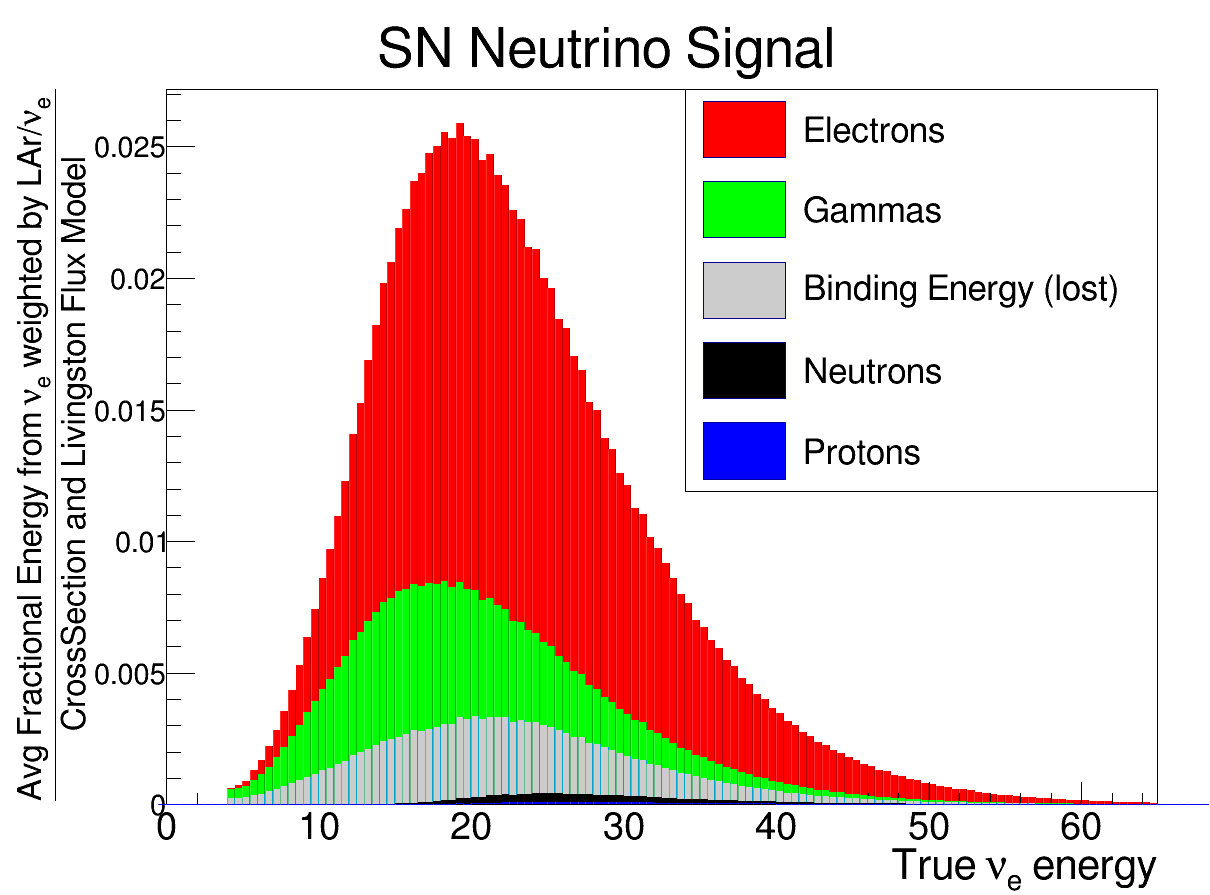
\includegraphics[height=2.0in]{snb-spectrum.eps}
\end{dunefigure}

\fixme{eps format not working (anne)}

The canonical reconstruction task is to identify the interaction channel, the neutrino flavor for \dword{cc} events, and to determine the four-momentum of the incoming neutrino; this overall task is the same for low-energy events as for high-energy ones.  The challenge is to reconstruct the properties of the lepton (if present), and to the extent possible, to tag the interaction channel by the pattern of final-state particles.

Calibration of absolute energy scale and understanding of energy resolution will be important for interpretation of the signal. We expect nominally $\sim$\num{20}\% resolution, although better would be desirable for resolution of supernova spectral features. Furthermore, a sample of data events of known properties with which to validate efficiencies of selection and reconstruction algorithms would be very valuable.

Given that the signal is expected to be uniformly distributed within the detector, absolute position resolution may not be critical (and events are likely to be widely separated in space for all but the very closest supernovae). However, good position resolution of photon detection is needed for good energy resolution, via correction for attenuation of charge during drift. Photon detectors in general may provide useful trigger information (and perhaps also ancillary energy information), so calibration of their time and light response is mandatory.

Absolute timing of events will be important for tracking the time structure of the burst. We expect that some $\sim$\num{0.1} fraction of a drift time ($<$\si{\ms}) will be sufficient for sensitivity to interesting physics signatures which vary in time. Therefore calibration of absolute timing response will be of value.

Understanding of backgrounds is also critical for reconstruction of low energy events, and for setting detector requirements. Small single-hit blips from $^{39}$Ar or other impurities may fake de-excitation gammas and also affect triggering. Backgrounds may be especially important for photon detectors.  Understanding of detector response to radiological backgrounds will therefore also be of value.

Potential calibration sources in this energy range include Michel electrons (studied in \dword{microboone}~\cite{bib:uBmichel}), which have a well known spectrum up to $\sim$50~MeV. One can also calibrate using $\gamma$, $\beta$ or neutron sources, which primarily give access to energies less than about 10~MeV. It is more challenging to find ``standard candles'' between 50~MeV and $\sim$\SI{100}{\MeV}, beyond cosmic-ray muon energy loss. \Dword{protodune} could potentially be a test bed for various calibration strategies. One can imagine also ancillary studies of detector response using detectors such as LArIAT~\cite{bib:LArIAT}, \dword{microboone}~\cite{bib:uB}, and SBND~\cite{bib:sbnd}. The ultimate calibration would be using a source of neutrinos from pion decay at rest, such as that available at the Spallation Neutron Source~\cite{bib:sns}, which have energies up to \SI{50}{\MeV} with a well-understood spectrum.

%KM notes: The Low Energy physics program includes searches for proton decay, detection of a core collapse supernova and signatures of dark matter.
%Many of the concerns of the low energy program are shared with  long baseline program, especially time dependent effects and identification of few MeV interactions. For example, supernova neutrinos have energies of about 20 MeV, but the energy is shared between neutron interactions, re-scattering of the electron, and de-excitation photons. So, a 20 MeV neutrino may be the combination of four 5 MeV sub-events. 
%The supernova (and other low energy physics) programs may have less stringent requirements (??10\% energy, position resolution??) but may be more susceptible to threshold effects.


%%%%%%%%%%%%%%%%%%%%%%%%%%%%%%%%%%%%%%%%%%%%%%%%%%%%%%%%%%%%%%%%%%
\section{Existing Calibration Sources} \label{sec:existsource}

All dedicated calibration systems must provide benefits outside of free, copious, and commonly used calibration sources, described in this section. DUNE will use particles from cosmic ray muons (Section~\ref{sec:cr}), neutrino-induced interactions (Section~\ref{sec:nuinduced}),  argon isotopes (Section~\ref{sec:ar39}) and information from instrumentation data  (Section~\ref{sec:inst}). Cosmic rays and neutrino-induced interactions provide commonly used ``standard candles'' like electrons from muon and pion decay, and neutral pions, which have characteristic energy spectrums. 

%%%%%%%%%%%%%%%%%%%%%%%%%%%%%%%%%
\subsection{Cosmic Rays }\label{sec:cr}
%- Tom Junk first draft}

Cosmic-ray events will provide the second-largest source of ionization charge in the DUNE \dword{fd},
after radiological decays.  Depending on the triggering strategy, cosmic-ray events may contribute the
most to the data volume from the far detector.  Starting from a predicted rate of four cosmic-ray muons
per square meter per day at the 4850' level at SURF~\cite{LBNEDOCDB9673}, we expect 
approximately \num{3}~million cosmic-ray particles per year for the four-module \dword{fd}.
A sample of \num{20000} cosmic-ray muons was simulated for a % single-phase 10~kt module 
\SI{10}{\kt} \dword{spmod} using the MUSUN
generator~\cite{Kudryavtsev:2008qh} and reconstructed using \dword{larsoft}.  This simulation draws muon
momenta from a pre-computed spectra with full angular and energy dependence given the local rock
composition and topography at the SURF laboratory.  The energy and angular distributions are given
in Ref.~\cite{LBNEDOCDB9673}.  The MUSUN generator only simulates single cosmic-ray muons;
muon bundles arising from high-energy atmospheric showers are not simulated yet.
The rates are uncertain at the level of 20\%.

Cosmic rays provide many critical measurements for DUNE, described in the following subsections. These include detector timing offsets, detector alignment, drift velocity, electron lifetime, relative channel calibrations, absolute gain,  electromagnetic response using decay electrons and $\pi^0$.
%These cosmic-ray events can be used to calibrate detector element locations, as well as the response of the detector to high-energy particles. 
Some events may be useful for some measurements and not others.  For example, detector alignment studies require muons that pass over the gaps between
\dwords{apa}, or pierce the \dwords{apa} or  \dwords{cpa}, while studying the electron drift and lifetime requires muons
that traverse the entire horizontal drift direction between the \dwords{apa} and \dwords{cpa}.  In the list of
possible measurements below, we estimate the daily rate of cosmic-ray muon events that can be used
and the requirements used to select these events.

%\subsubsection{Possible Measurements}
%%%%%%%%%%%%%%%
\subsubsection{Detector Timing Offsets}

A measurement of the global time offsets between the TPC wire readout and the photon detectors
and external sources of timing information (such as external muon counters), can be made
with tracks that cross through the \dword{apa} volumes.  Hits on either side of the \dwords{apa} drift in opposite
directions and thus a constrained fit for a track to line up on both sides of an \dword{apa} requires the
time of the event to be correct.  Hits that drift from locations close to the \dwords{apa} are minimally
affected by space charge and other field distortions.

Approximately six non-showering muons are estimated to pierce each \dword{apa} per day.  This number
is the nine muons per day crossing a vertical gap, which is estimated in the next section, multiplied
by (\SI{2.5}{\m})/(\SI{3.6}{\m}), the ratio of the width of an \dword{apa} to the drift distance.  Timing offsets can therefore
be measured in under a week on an \dword{apa} by \dword{apa} basis, and a global timing offset with less than a day's worth
of data.
 
 %%%%%%%%%%%%%%%%%
\subsubsection{Detector Alignment}

The 150 \dwords{apa} in a \dword{spmod} are expected to be rigid bodies that are assembled to
precise mechanical tolerances.  The requirements for physics analyses however often exceed 
mechanical tolerances that can be achieved, especially after cooldown.  Straight tracks that cross
from the volume of liquid argon that is read out by one \dword{apa} into the volume read out by another \dword{apa}
give, by steps in their apparent positions and angles, constraints on the relative positions and angles
of the \dwords{apa} as they are situated in the detector.   A full alignment campaign using cosmic rays will
find the minimum of a $\chi^2$ function that depends on the measured track segments, positions and angles of
the \dwords{apa} and  \dword{cpa} panels, and includes any external constraints such as mechanical surveys, along with
realistic uncertainties.  Examples of cosmic-ray alignment campaigns can be found from 
ATLAS~\cite{LacuestaMiquel:2015ksh,Moles-Valls:2014wza}, CMS~\cite{Chatrchyan:2009km}, ALICE~\cite{Aamodt:2010aa},
In the following discussion, the $y$ axis is vertical, the $x$ axis points along the electric field,
and $z$ points approximately along the beam direction.

Given experience from the \dword{35t}, we predict
that the precision on the width of a vertical gap between two neighboring \dwords{apa} is
\begin{equation}
\sigma_{\Delta z} \approx \frac{1.79\times 10^{-1}~{\rm{cm}}}{\sqrt{N_{\rm{tracks}}}},
\end{equation}
where $N_{\rm{tracks}}$ is the number of cosmic-ray muon tracks used to make the measurement,
and the precision on offsets in the \dword{apa} positions along the drift direction (aplanar steps) is
\begin{equation}
\sigma_{\Delta x} \approx \frac{5.83\times 10^{-2}~{\rm{cm}}}{\sqrt{N_{\rm{tracks}}}}.
\end{equation}
Naively taking the top half of an \dword{apa} as a separate measurement from the bottom half and using these
precisions to estimate angular resolutions.  We thus estimate
\begin{equation}
\sigma\left(\frac{d\Delta z}{dy}\right) \approx \frac{\sqrt{2}\sigma_{\Delta z}(N_{\rm{tracks}}/2)}{3~{\rm{m}}}
\approx
\frac{1.19\times 10^{-3}}{\sqrt{N_{\rm{tracks}}}}
\end{equation}
and
\begin{equation}
\sigma\left(\frac{d\Delta x}{dy}\right) \approx \frac{\sqrt{2}\sigma_{\Delta x}(N_{\rm{tracks}}/2)}{3~{\rm{m}}}
\approx
\frac{3.89\times 10^{-4}}{\sqrt{N_{\rm{tracks}}}}.
\end{equation}


The numbers of tracks available to make these measurements depends on the energies, positions, and angles
required.  The energy of muons is required to be less than \SI{485}{\GeV}, the critical energy in \dword{lar},
above which bremsstrahlung and pair production dominate the energy losses over ionization.  Tracks
that have too many electromagnetic showers along their lengths cannot be used for alignment, though
analyses that use track sections that are locally straight might be able to recover a fraction of these.
We require that at least \num{20} collection-plane wires are hit by a track on either side of a vertical gap, providing
enough space points to measure the parts of the track on either side of the gap.  Saturation of the \dword{adc}
is an issue for some measurements but should affect alignment studies less than lifetime and signal
strength calibrations, so the geometrical requirement is currently estimated to be sufficient.
Given the full simulation and these requirements, approximately nine muons that can be used for alignment
pass through the argon over a vertical gap every day.  Horizontal gaps between \dwords{apa} that are stacked
vertically are shorter, but given the dominantly vertical direction of the incident muons are easier
to hit per unit area.  We estimate that ten muons per day pass through a horizontal gap and can be
used for alignment.

The cathode planes provide additional alignment tasks that can be addressed with cosmic rays.
Because there are six cathode plane panels per \dword{apa}, there are more alignment parameters to consider.
Similarly to the ICARUS experience, the volume on both sides of the cathode planes is active, and charge
drifts in opposite directions on the sides of the cathode.  Thus, if a cathode plane element is displaced
in $x$, a track that pierces it will appear to extend beyond the physical location.  We assume the
same rate of cosmic-ray muons piercing the cathode planes per unit area as for the \dword{apa} planes, which
means one muon per day per cathode-plane panel is expected.  A full alignment with \SI{1}{\m$^2$} pixels of the
ICARUS cathode took roughly six months of data, and it is reasonable to expect a similar amount of time
needed to fully align the cathode panels of DUNE.

One of the main drivers of precise alignment is to be able to use multiple scattering in order to
measure muon momentum for muons that escape the detector before stopping.  
This analysis has been performed by ICARUS~\cite{Antonello:2016niy} and by \dword{microboone}~\cite{Abratenko:2017nki}.
Residual uncertainties in the cathode plane flatness in were the limiting systematic uncertainties
in the ICARUS measurement.

%%%%%%%%%%%%%%%%
\subsubsection{Drift Velocity and TPC Size}

Tracks that pierce both an anode plane and a cathode plane in DUNE are particularly valuable. %because
The difference in arrival times of the drifting charge gives the total drift distance divided by the
drift velocity, assuming one of these quantities gives a measurement of the other.

%%%%%%%%%%%%%%%%
\subsubsection{Electron Lifetime}

Tracks that leave ionization at a variety of different distances from the anode provide a sample
with which to measure the electron lifetime.  Two similar methods have been used.  In the
first, track charge deposits $dQ/dx$ are measured, the highest and the lowest are ignored because
the tail of the Landau offers less information than the core, and an exponential is fit on a 
track-by-track basis.  The track-by-track electron lifetime is then averaged over many such tracks
(the reciprocals are in fact averaged to help remove biases due to asymmetric uncertainties).  In
the second method, a single exponential is fit to the sum of the measured $dQ/dx$ values for many tracks.
Examples of these methods can be found from ICARUS~\cite{Antonello:2014eha}, 
\dword{microboone}~\cite{Meddage:2017lxo,MICROBOONE-NOTE-1026-PUB}, as well as in the \dword{35t} and
the LArIAT detectors.  Extrapolating from the ICARUS precision on $\lambda = 1/\tau$, we expect
that each cathode-anode piercing track will provide a $\pm 30$\% measurement of the lifetime
at a lifetime of \SI{3}{\milli\s}.

If one requires tracks to pierce both an anode plane and a cathode plane and have an energy between \SI{20}{\GeV}
and \SI{400}{\GeV} in order to be straight and non-showering, then the rate is five per day per drift volume
on one side of an \dword{apa}.  If one further requires that the muon pierce one of the six cathode panels
directly opposite to the \dword{apa} it pierced, then the rate falls to \num{1} per day.  \dword{adc} saturation is not
a concern for tracks that traverse the entire drift length.

%%%%%%%%%%%%%%%%
\subsubsection{Relative Channel Calibration}

Channel-to-channel gain variations can be tested with large samples of cosmic-ray muons.  The rate at
which a single collection-plane channel records useful data from cosmic-ray muons is very similar to that
for the vertical gaps between \dwords{apa}, or roughly ten per day.  In this case, \dword{adc} saturation is a concern,
but traversing forty collection-plane wires in the \SI{6}{\m} height as per the angular requirement for alignment
should keep the hits from saturating the \dwords{adc}.

Nonetheless, a comparison of the gains of faraway channels requires averaging over a large ensemble
of cosmic-ray muons, as the muons will have different energies and thus different $dE/dx$ values,
and given their dominant vertical directions, each will hit only a portion of an \dword{apa}.  A high-precision
calibration of each channel's relative gain will likely take on the order of months, depending
on the track-to-track variation in measured $dQ/dx$ values which affects the rate of convergence
of the average.

%%%%%%%%%%%%%%%%
\subsubsection{Absolute Gain Calibration with MIPs}

A measurement of the MIP scale in the DUNE Far Detector will be more challenging, as the $dE/dx$
distribution depends on the energies of the incident muons.  With a model of the energies,
one can find the distribution of $dQ/dx$ values and fit it with a floating global gain value
and uncertainties in the parent energy distribution to obtain a global scale.  This method
is subject to systematic uncertainties arising from the energy scale of the incident muons.

%%%%%%%%%%%%%%%%
\subsubsection{Electron Response Calibration from Michel Electrons}

Stopping $\mu^+$ particles will produce Michel electrons with a known energy spectrum which can
be used to calibrate the response of the detector.  An example analysis of Michel electron
reconstruction is available from \dword{microboone}~\cite{Acciarri:2017sjy}.  This analysis is sensitive
to the collection of energy deposited by bremsstrahlung photons which Compton-scatter a short distance away from
the Michel electron, and is useful in tuning up reconstruction as well as the simulation.  Approximately
\num{30} muons per day are expected to stop in a \SI{10}{\kt} module.

%%%%%%%%%%%%%%%%
\subsubsection{Electromagnetic Energy Scale from $\pi^0$ Decays}

An estimate of the rate at which cosmic-ray muons produce $\pi^0$'s is of the order of one per \num{1000}
cosmic rays.  The ICARUS experiment performed an analysis of \num{212} candidate $\pi^0$ decays
from the 2001 Pavia surface test run~\cite{Ankowski:2008aa}. 
%The rate is expected to be low in the far detector, and may be overshadowed by atmospheric neutrino interactions. %% KM our other table says 300 atm nu induced vs. 3000 here

% Table or text about rates of each category of event. 

%%%%%%%%%%%%%%%%
\subsubsection{Limitations}

As described in Refs.~\cite{LacuestaMiquel:2015ksh,Moles-Valls:2014wza}, alignment of detectors using
only cosmic-ray muons leaves some combinations of uncertain parameters only loosely constrained.
These are labeled ``weak'' directions in the citations above.  While the DUNE far detector geometry is
significantly different from a collider detector, similar weak directions will appear in the cosmic-ray
alignment campaign.  Distortions of the detector that preserve the gap widths and do not shift
the \dwords{apa} in $x$ near the gaps relative to one another will be difficult to measure with cosmic rays.
These distortions include global shifts and rotations in the locations of all detector elements,
and crumpling modes where the edges of the \dwords{apa} hold together but angles are slightly different
from nominal.  An example of such a distortion is shown in Figure~\ref{fig:crumplemode}. 

\begin{dunefigure}[Sample distortion that may be difficult to detect with cosmic rays]{fig:crumplemode}{An example of a distortion that may be difficult to detect with cosmic rays.  The \dword{apa} frames are shown as
rotated rectangles, as viewed from the top.}

\includegraphics[width=0.8\textwidth]{apacurtainalign.png}
\end{dunefigure}

\fixme{better to make the label match the figure file name, e.g., fig:apacurtainalign. (anne)}
There is a global degeneracy between the drift velocity and the drift distance scale in the \dword{fd},
as measured with cosmic-ray muons.

The uncertainty in the energy spectrum of cosmic-ray muons is a limitation on the global \dword{mip}
calibration using these events.

Some of the measurements described above, such as the channel-to-channel gain uniformity and the
cathode panel alignment, are estimated to take months of data.  We will initially assume that
the calibration parameters are constant and average over the data as it comes in, and only after
larger data samples have been accumulated can more differential measurements be made, such as
constraining time dependence of channel gains and spatial dependence of the electron lifetime.

%%%%%%%%%%%%%%%%
\subsubsection{Remaining Studies}

Each of the analyses described here requires a full effort to carry to completion with data.
Estimates of sensitivity using simulated data can be used to estimate the levels of precision expected
as functions of time.  
%Combinations of information from cosmic-ray events and other calibration sources, such as a laser system, will reduce the total uncertainties.

%%%%%%%%%%%%%%%%%%%%%%%%%%%%%%%%
\subsection{Neutrino-induced interactions }\label{sec:nuinduced}
%- Vitaly draft; editing by Kendall}

%{\it stopping protons?} \\

Beam and atmospheric neutrinos and antineutrinos will provide interactions useful for certain calibrations of the \dword{fd}.%DUNE FD. 
Both sources of neutrinos will produce CC and NC events, where CC interactions will also provide a muon and electron in the event. Table \ref{table:nu-rates} summarizes event rates from different neutrino sources. Neutrinos (or antineutrinos) will produce muons outside and inside the detector that can be tagged as partly or fully contained events. Fully contained events provide more information since the total energy (and the total muon energy) can be reconstructed from the muon range and $dE/dx$. 

\begin{dunetable}[Atmospheric and beam neutrino and antineutrino event rates per year]{cc}{table:nu-rates}
{Atmospheric~\cite{cdr-2} and beam neutrino and antineutrino event rates per year in \SI{40}{\kt} fiducial mass of the \dword{fd}. The beam-rock interaction rate is for the front (beam direction) face of the \dword{detmodule} %DUNE cryostat 
only; additional interactions will occur along the side.} % of the cryostat. }
%\begin{center}
%\begin{dunetabular}{|c|c|}
%\hline
Fully contained atmospheric $e$-like & $1.6\times10^{3}$ \\ \colhline
Fully contained atmospheric $\mu$-like & $2.4\times10^{3}$ \\ \colhline
Partly contained atmospheric $\mu$-like & $7.9\times10^{2}$ \\ \colhline
CC or NC atmospheric $\pi^0$ & $300$ \\ \colhline
CC or NC atmospheric $K^+$ & $20$ \\ \colhline %(K+) is less than 1% of events (0.7-0.8%), so we may have 20 per year in 40 kt. This is from Andy’s Blake LBNE note 8836. KM couldn't find reference
Beam induced, rock\cite{bib:docdb6628} $\mu$-like & $2.8-5.6\times10^{3}$ \\ \colhline
Beam induced, Ar (signal) $\mu$-like & $2.8\times10^{3}$ \\
%\end{tabular}
%\end{center}
\end{dunetable}
 
 %%%%%%%%%%%%%%%%
 \subsubsection{Possible Measurements}
   
%Beam and atmospheric neutrinos will provide interactions useful for certain calibrations of the DUNE FD. Both sources of neutrinos will produce CC and NC events, where CC interactions will also provide a muon and electron in the event.
%with CC events resulting in better energy reconstruction of the whole event and in muons or electrons useful for calibrations. 

%However, the calibration use of some of the  the use of fully contained beam-Ar induced events must be treated with care as these events are  The use of beam-induced electron-like events is limited because they also represent signal events in the detector. 

%I think, the kaon production (K+) is happening in less than 1% of events (0.7-0.8%), so we may have 20 per year in 40 kt. This is from Andy’s Blake LBNE note 8836.

Although cosmic-ray muons have much higher event rates compared to atmospheric or beam neutrinos, neutrino CC events have a few advantages.  Beam events will complement cosmic-ray muon calibration, in particular at near-horizontal directions ($\cos\theta < 0.3$) where cosmic-ray muons are absent. Neutrino-induced muons will help with testing the \dword{apa} alignment.  However, only high-energy muons will provide accurate measurements since low-energy muons may undergo large scattering.

Both partly and fully contained muon events will give us a sample of electrons from muon decay (for electron ID and shower calibration). In addition, events with negative muon capture, which emit protons and neutrons will be a valuable sample. This topology is relevant to various rare event searches, like nucleon decay, which rely on separating positive kaons from a sub-sample of negative kaons. Beam-induced events will also provide a small but valuable $\pi^{0}$ sample for energy scale.

Beam-induced events may also be used for reconstruction validation in certain circumstances. A muon or electron CC neutrino event tagged by a clear identification of a muon or an electron (via a shower) will allow us to test lepton identification. There should be no other lepton emerging from the primary vertex in such events so any lepton found by the reconstruction (not coming from a secondary hadronic decay).  Neutrino events will have more predictable outcomes and topologies compared to higher energy cosmic-ray muon events, and have a higher probability of producing low-energy hadrons.  Although some of these events are signal for the long baseline program and will not be used directly for calibration, one can test of particle identification using beam events for rare event searches, e.g. nucleon decay or neutron-antineutron oscillations.

%Due to a small number of tracks related to neutrino interactions, the reconstruction of tracks and showers from these events should not be difficult. Hence $\pi^{0}$ mass reconstruction and energy spectrum of electrons from muon decay will provide additional inputs to the energy calibration of the FD.

 %Neutrino events will complement cosmic-ray muon calibration, in particular at near-horizontal directions ($\cos\theta < 0.3$) where cosmic-ray muons are absent. 

%%%%%%%%%%%%%%%%
\subsubsection{Limitations}

The main limitation for using neutrino events is their low rate. Any calibration required on day-to-day basis is impossible with these events. It will also be difficult to get accurate results for individual TPCs within the \dword{fd}. 
%However, overall alignment of APAs (changes are not expected here on short time-scales), muon $d E /d x$, shower calibration from muon decay electron spectrum, energy calibration from $\pi^{0}$ mass and particle ID reconstruction tests can be performed.
%Due to low rate of neutrino-induced events, their application for (relative) calibration is quite limited. However, they may provide supplementary information on energy calibration ($d E /d x$ and showers) and be useful for particle ID reconstruction tests. 

We also note that the beam from LBNF at Fermilab will probably be ready a year or two after the commissioning of the first \dword{detmodule}. Hence beam neutrinos may not contribute to the first module calibration at the beginning of running.

%%%%%%%%%%%%%%%%
\subsubsection{Remaining Studies}

Discussion on suitability of beam and atmospheric neutrinos to calibrations will benefit from full simulations of these neutrinos including reconstruction within \dword{larsoft}. For atmospheric neutrinos this has been done in connection with the background for nucleon decay searches but the information relevant to calibrations has not been analysed. Similar studies are required for beam neutrinos to better understand their suitability for calibrations.

%%%%%%%%%%%%%%%%%%%%%%%%%%%%%%%%
\subsection{Argon 39}
\label{sec:ar39}
%- written by Mike Mooney; major editing by Sowjanya}
%Purpose: Primary: Model validation (confirm space charge is sensible after other systems?). Potential main measurement: Lifetime? Because it is everywhere. 
The reconstructed energy spectrum of ${}^{39}$Ar beta decays can be used to perform a variety of in-situ and ex-situ measurements of detector effects relevant for particle reconstruction in the DUNE far detector. The ${}^{39}$Ar beta decay rate in natural (atmospheric) argon is about \SI{1}{\becquerel\per\kilo\gram}, so $O(\mathrm{50k})$ ${}^{39}$Ar beta decays are expected in a single \SI{5}{\milli\s} event readout in an entire \SI{10}{\kt} \dword{detmodule}. The ${}^{39}$Ar beta decay cut-off energy is \SI{565}{\keV} which is close to the energy deposited on a single wire by a \dword{mip}. Another useful feature of ${}^{39}$Ar beta decays is that they are uniform in the drift direction.

%%%%%%%%%%%%%%%%
\subsubsection{Possible Measurements}
Given that the large number of ${}^{39}$Ar beta decays are present through out the volume of the detector, this method allows for a fine-grained (spatially and temporally) electron lifetime measurement in the \dword{fd}. %DUNE far detector.
 It can also provide other necessary calibrations, such as measurements of wire-to-wire response variations and diffusion measurements using the signal shapes associated with the beta decays, and could serve as an online monitor of electric field distortions in the detector by looking at the relative number of decays in the detector near the edges of the \dword{lartpc}. The viability of this method has already been demonstrated with \dword{microboone} data (results expected to be released publicly sometime later this year), both for \dword{microboone} and a projection to conservative operating conditions of the \dword{fd}. %DUNE far detector. 

\begin{dunefigure}[Impact of detector effects on ${}^{39}$Ar beta decay electron energy spectrum]{fig:ar39}
{Illustration of the impact of different detector effects on the reconstructed ${}^{39}$Ar  beta decay electron energy spectrum for decays observed in the \dword{spmod}.  On the left are examples of the reconstructed energy spectrum for various different electron lifetimes, as well as the nominal ${}^{39}$Ar  beta decay spectrum (corresponding to an infinite electron lifetime).  On the right are examples of the reconstructed energy spectrum when the true recombination model is different from the one assumed in energy reconstruction (varying the $\alpha$ parameter of the modified Box model, $\mathcal{R} = \ln(\alpha + \xi)/\xi$, where $\xi = \beta\frac{dE}{dx}/{\rho}E_{\mathrm{drift}}$ and with fixed $\beta = 0.212$) and the electron lifetime is infinite.  All curves have been normalized to unit area.}
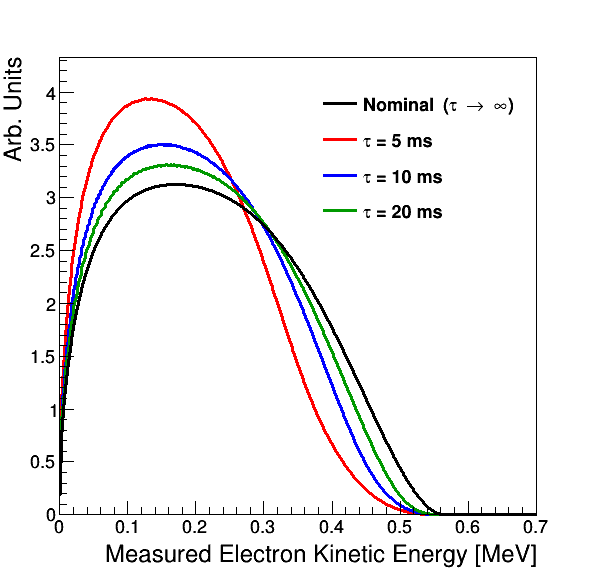
\includegraphics[width=.49\textwidth]{Ar39_energyPlot_DUNESPFD_lifetime.png}
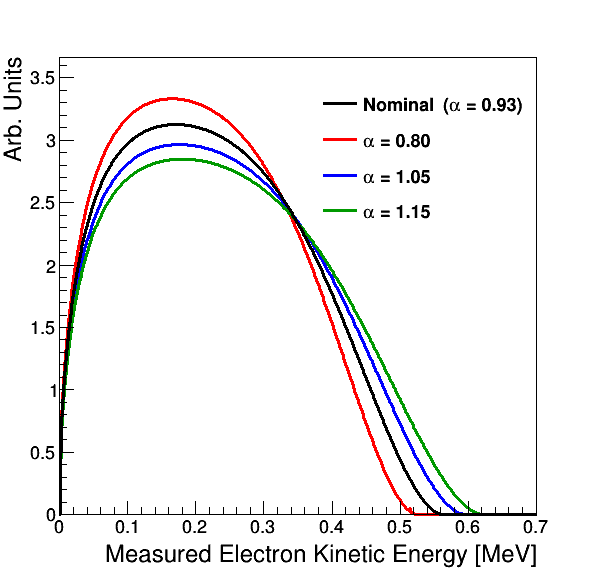
\includegraphics[width=.49\textwidth]{Ar39_energyPlot_DUNESPFD_recomb.png}
\end{dunefigure}

Using the fact that the ${}^{39}$Ar beta decays are uniformly distributed in the drift direction, one is able to precisely determine the expected reconstructed energy spectrum for a given set of detector response parameters. This can be done independently of using timing information (e.g.~from prompt scintillation light). As an example, one can use the reconstructed ${}^{39}$Ar beta decay energy spectrum to constrain primary detector response parameters such as the electron lifetime and recombination simultaneously. Figure~\ref{fig:ar39} illustrates the different possible reconstructed ${}^{39}$Ar beta decay electron energy spectra one might see after correcting for all other detector effects except for electron lifetime, for ${}^{39}$Ar beta decays occurring in the \dword{spmod}. Also shown in Figure~\ref{fig:ar39} is the impact of varying the true recombination model from the one assumed in energy reconstruction of the ${}^{39}$Ar beta decay electron, with infinite electron lifetime. The impact on the reconstructed energy spectrum is very different for the two detector effects, allowing for simultaneous determination of both quantities.

One important consideration is whether or not the \dword{fd} \dword{daq} system can provide the necessary rate and type of data in order to successfully carry out this calibration at the desired frequency and level of spatial precision. From studies at \dword{microboone}, an estimate of the number of decays necessary to carry out a percent-level calibration of electron lifetime is $O(\mathrm{250k})$. This means that in order to make a single measurement of electron lifetime in an entire \dword{detmodule}, one would only need roughly five readout events (note $O(\mathrm{50k})$ decays per readout window per \SI{10}{\kt} \dword{detmodule}). However, one must also allow for the electron lifetime to spatially vary throughout the entire \SI{10}{\kt} \dword{detmodule}; it is not clear how much variation one should expect in a detector of this size. A reasonable (though arbitrary) level of granularity to serve as a benchmark is one measurement per $\mathrm{m}^{2}$ (recall that the measurement is averaged over the drift direction, and thus is made in only two dimensions). Measurements with this level of granularity would require $O(\mathrm{100k})$ readout events (\SI{5}{\milli\s} in length). This results in a requirement of roughly \SI{1}{\hertz} for minimum-bias event trigger rate in order to perform this calibration once per day, as is done at other \dword{lartpc} detectors that are currently operating. 
%The 1~Hz rate could either be obtained through hardware triggers issued at 1~Hz or hardware triggers issued at a higher rate and then pre-scaled in software. Minimum-bias triggers are sufficient as there are plenty of ${}^{39}$Ar beta decays in every event readout. Taking minimum-bias triggers at 1~Hz. 
This leads to a data rate of roughly \SI{4}{\giga\byte\per\s} for an entire \SI{10}{\kt} \dword{detmodule} without zero suppression. With zero suppression, using a threshold based upon noise levels expected at the \dword{fd} (\num{400} to \num{500} electrons for collection plane wires), one arrives at roughly \SI{5}{\mega\byte\per\s}. The data rate for the zero-suppressed case takes into account the use of a three wire by \num{40}~time tick window for each candidate decay in a single plane; this window was determined to be optimal for studies at \dword{microboone}, and would only be tweaked slightly for DUNE. 

%%%%%%%%%%%%%%%%
\subsubsection{Limitations}
%Strongly threshold driven, or noise issues. Translated to MeV limit. What is it? How does it change under noise assumptions? Before call it a big option, confirm noise issues. Is it disastrous?
There are several factors that impact the observed charge spectrum from 
${}^{39}$Ar beta decays such as electronics noise, electron lifetime and recombination fluctuations. The effect of electron lifetime is more pronounced in dual phase due to the longer drift distance requiring the measurement be carried out more precisely. Also for this method to work, noise level must not be too high (requires less than \num{1000} e$^{-}$\,ENC) and a precision noise measurement is required. Another limitation of this method is that it mainly probes regions closer to the anode; extrapolations to other regions in drift requires the electron lifetime be constant across the volume. One can use cosmic rays in these regions to mitigate this limitation, but a lower electron lifetime can complicate this process. 

Note that the \dword{daq} rates estimated previously does not take into account the need to save enough data on the induction planes which will have higher noise level. In this case, it might be necessary to save many induction plane wires for a candidate ${}^{39}$Ar beta decay found on a single collection plane wire, leading to a much higher data rate (factor of $O(100)$ higher). One can get around this requirement by making the electron lifetime measurement strictly in the $z$ direction (by far the longest dimension of the detector, and thus most interesting to probe spatial variations of electron lifetime), or by introducing a tighter requirement on the reconstructed charge threshold for the induction planes.

%%%%%%%%%%%%%%%%
\subsubsection{Remaining Studies}
Currently, the plan is to study this calibration technique in more detail with first data from \dword{protodune}, well in advance of first operations with the \dword{fd}, to understand lessons learned and challenges for DUNE.  

%SG: don't want to include the following, extra stuff from MM:
%Characterizing the raw ${}^{39}$Ar  beta decay charge spectrum in a smaller device (capable of tagging light associated with individual ${}^{39}$Ar  beta decays in order to correct electron lifetime on a decay-by-decay basis) ahead of first operations of the DUNE far detector will increase the precision of the electron lifetime measurement at DUNE.  Such a device should be placed deep underground in order to ensure effectively zero contamination from charge or light of cosmogenic origin. 
%Notes from SG :Some specific studies that can help here are: 1. Simulation studies to understand the limitation in the usability of the source if we do not achieve the noise levels we want.  2. What is the dependence of electron lifetime on signal? Simulation studies to understand the impact of electron lifetime for DUNE. Can one take low purity and high purity data at \dword{microboone} and do this study? 3. Continue developing techniques to use this source for calibration studies at uB and \dword{protodune}. This will validate the analysis techniques and benchmarks what can be achieved from this source. 4. Take the techniques developed at uB/\dword{protodune} and understand what parameters/variables need to be tuned to extrapolate the techniques to DUNE and assess (with simulation studies) what impact those variables will have on the results. 5. Any \dword{daq} related studies to mitigate the issues with high rates?

%%%%%%%%%%%%%%%%%%%%%%%%%%%%%%%%
\subsection{Instrumentation and Monitoring Data }
\label{sec:inst}
%- written by Sowjanya}
There will be several instrumentation and detector monitoring devices that will provide valuable information for calibration. %In addition to instrumentation data, there will also be detector monitoring data that can provide useful information for calibrations and physics and also inform about the stability of various detector variables.
The cryogenic instrumentation and detector monitoring effort for DUNE is centrally led by the Cryogenic Instrumentation and Slow Controls (CISC) consortium. These instrumentation devices include liquid argon temperature monitors, liquid argon purity monitors and gaseous argon analyzers, and cryogenic (cold) and inspection (warm) cameras. There are other instrumentation devices such as drift \dword{hv} current monitors and external charge injection systems that will be useful for calibrations that will be led by the high voltage and TPC cold electronics consortia, respectively. The computational fluid dynamics (CFD) simulations play a key role for calibrations initially in the design of the cryogenics recirculation system and later for physics when the CFD simulations are validated using cryogenics instrumentation data. This section provides a brief description of possible measurements with various instrumentation devices and also what detector monitoring data will be useful for calibrations.

%%%%%%%%%%%%%%%%
\subsubsection{Possible Measurements}
Electro-negative contaminants such as oxygen and water in the liquid can absorb signal electrons created from the ionization of argon atoms. The gas analyzers can be used for measuring these contaminants in the liquid. There is plan to deploy gas analyzer system for DUNE that will be capable of taking measurements at multiple points around the cryogenics system. In addition to gas analyzers, purity monitors provide quick measurements of liquid argon purity by measuring electron lifetime (through anode to cathode charge ratio) in a small space typically less than a meter. The purity monitor measurements are especially useful during detector commissioning and intial operations when cosmic ray data will not be availble to perform more detailed studies. Electron lifetime correction is an important step in calorimetric reconstruction and can also impact many other parameters such as electron recombination and track reconstruction. There is a plan to deploy three purity monitors inside the cryostat and some in the inline filters of the argon purification system. 

There will be several thermometers, both individual sensors, vertical temperature gradient monitors (both static and movable), that will be installed through out the volume of the cryostat that will provide liquid argon temperature measurements with a precision goal of \SI{5}{\milli\kelvin}. The biggest impact of liquid argon temperature is on the electron drift velocity through the drift coordinate which in turn affects detector fiducial volume. Drift velocity can also impact measurements like electron diffusion which rely on a measurement of the drift velocity. Both temperature and purity monitor data will be critical to validate the liquid argon flow model. Validation of the fluid flow model using instrumentation data will give confidence in using the model for projections for physics to understand impact of various liquid flow properties. In addition to instrumentation data, the cryogenics system data such as liquid argon contamination levels, temperatures and various flow parameters will be continuously monitored and recorded providing additional information for calibrations.

DUNE plans to deploy both cryogenic cameras and inspection cameras. The cryogenic cameras will be used to look for \dword{hv} activity, especially breakdowns. The inspection cameras will be used to monitor the health of the detector components and to visually diagnose in case of issues. Both of these data will be useful for calibrations to understand any electric field anamolies or unexpected drift field responses. Additionally, to further monitor and diagnose high voltage issues, installing devices such as current monitors will be useful to diagnose or characterize the field cage. The experience from \dword{microboone} using a source meter to continuously monitor pick off point voltage with respect to the ground has helped the collaboration diagnose \dword{hv} problems.

%%%%%%%%%%%%%%%%
\subsubsection{Limitations}
While purity monitors have practical advantages in terms of speed of measurement and the ability to measure low electron drift-lifetimes before tracks can be reconstructed, purity monitor measurements are very localized and do not necessarily reflect any purity variations in the cryostat. Also, purity monitors typically measure the effect of the contaminants at a lower electric field. In fields above about \SI{200}{\V/\cm}, the drift-field increases the speed of the drift electrons and this can lead to a different electron capture cross section on the contaminants for the purity monitor and the drift-electrons in the TPC. Additionally, purity monitors also have limited lifetime so it is important to be aware that their measurements will not be available for the entire lifetime of the experiment. To mitigate this, \dword{microboone} has developed a nearline purity monitoring system that uses a statistically sufficient sample to make a purity measurement using cosmic ray muons. Developing similar techniques for DUNE will be very useful. The low cosmic rate might be an issue here but one may be able to make a less frequent nearline measurement. In the case of temperature monitors, achieving the needed precision is a challenge and will impact how well one can validate the fluid flow model using temperature data. 

%%%%%%%%%%%%%%%%
\subsubsection{Remaining Studies}
The remaining studies one can do prior to TDR are the following:
\begin{itemize}
\item A validation of the fluid flow model using instrumentation data at \dword{protodune} will be very informative and valuable for DUNE. 
\item Implement a nearline purity monitoring using cosmic rays (like \dword{microboone}) to understand the challenges of implementing such a system in a larger scale detector.
\item Using current CFD simulations understand the range of variation for various flow-related parameters (e.g., overall temperature variation in the cryostat, overall impurity variation across the detector) and propagate those variations to calibration and understand the impact on physics.
\item CFD studies to understand how argon flow can impact space charge and ion accumulation (both positive and negative ions). This will be especially critical for the dual phase design due to the liquid-gas interface.
\end{itemize}

%%%%%%%%%%%%%%%%%%%%%%%%%%%%%%%%%%%%%%%%%%%%%%%%%%%%%%%%%%%%%%%%%%%%%%
\section{External Measurements Relevant to Calibration }\label{sec:extcalib}
%- David C.? Stephen P? Kendall outline}
%Role of external measurements, previous LAr TPCs or test stands. External data provides dedicated physics parameter measurements (e.g. recombination) as well as overall validation that the TPC response model is complete. 
%Previous experiments: ICARUS, ProtoDUNE, ArgoNeuT, SBND, uB, LAriAT. 
%Also test stands like the Field Response Calibration Device (Chao's work) 
%The near detector will provide similar information as previous experiments. At time of writing, the near detector configuration is not determined. 
This section presents a summary of available measurements performed with \dword{lartpc} detectors that are relevant for the \dword{fd} calibration strategy. Upcoming measurements from currently operational and future detectors in the Fermilab Short Baseline Neutrino program, and from the \dword{protodune} detectors %prototypes 
at CERN are also discussed. 

%%%%%%%%%%%%%%%%%%%%%%%%%%%%%%%%%%%%%
\subsection{Measurements of detector response model}
%Measurements of recombination, lifetime, diffusion, alignment. Photon system.%Field response
Energy loss by charged particles traversing liquid argon leads to ionization and scintillation signatures which are eventually recorded as signals in the detector. The physics processes which lead to the formation of these signals and the detector effects which impact their propagation must be carefully understood in order to perform adequate calibrations which ultimately impact the detector's energy response. A wide range of measurements for such effects has been performed either with R\&D test-stands or neutrino detectors. These measurements, with brief discussions pertaining to their relevance, are presented in this section.

%%%%%%%%%%%%%%%%%%
\subsubsection{Scintillation Light}
Light detection plays an important role in the analysis of neutrino interactions with \dword{lartpc} detectors. Scintillation light provides essential timing information which complements the slow-drifting ionization signal, and can be used to further improve measurements of calorimetric energy loss and particle-identification. Extensive studies of the properties of scintillation light in \dword{lar} have been performed with numerous experiments, with significant contributions to knowledge in this subject coming from dark matter as well as dedicated test-stand experiments such as those performed at Fermilab's PAB. \fixme{write out}

External measurements of light quenching due to impurities such as nitrogen~\cite{bib:scintillationN2} and methane~\cite{bib:scintillationCH4} are useful in determining absolute light yields and the ratio of prompt to late scintillation light ratios. Measurements of the properties of TPB, \fixme{write out} used to shift argon scintillation light to the visible spectrum, as well as Rayleigh scattering and ionization-dependent light yields are all important for proper simulation of the light response in \dword{lartpc} detectors. In addition to studies that impact the calibration of detector effects, a large amount of work has been and is being performed addressing how light yield, performance, and light collection uniformity impact different photon detection %PDS 
technologies. Examples of such measurements, many of which are performed at Fermilab's PAB facility, can be found in references~\cite{bib:arapuca},~\cite{bib:attnlength}, and~\cite{bib:lightguide}.

%%%%%%%%%%%%%%%%%%
\subsubsection{Ionization Electrons}
Many detector effects impact the ionization signals ultimately recorded by the TPC wires. The significant impact of these effects is in large part due to the slow drift of ionization electrons in the TPC, of order $\mathcal{O}(1)$ mm/$\mu$s. Detector effects impact ionization electron signals both by quenching the total ionization charge, as well as by producing local variations in detector response. These in turn lead to relative and absolute energy scale variations which impact energy resolution and bias respectively. Careful calibration of these effects can significantly improve the energy resolution and particle identification performance which are essential in order to achieve DUNE's physics goals.

The major effects which impact detector response to ionization energy loss are listed below, together with relevant measurements of these effects.
\begin{enumerate}
\item \textbf{Ion Recombination} Ionization electrons in the vicinity of positive argon ions can recombine, quenching the TPC signal. This detector effect is dependent on the concentration of $e^-$-Ar ion pairs produced and the time such pairs spend in close proximity. The first is determined by the local $dE/dx$ energy loss, and the second by the strength of the electric field. Recombination quenches ionization signals by $\sim$50\%, causing one of the most significant biases in collected signals. Measurements of ion recombination with stopping muons and protons of energy ranges relevant to \si{\GeV} $\nu$-Ar interactions have been performed by the ICARUS~\cite{bib:ICARUSrecomb} and ArgoNeuT~\cite{bib:ARGONEUTrecomb} experiments. These measurements are performed in a range of $dE/dx$ which spans from \num{2} to \SI{25}{\MeV\per\cm}, at field strengths in the \num{0.2} to \SI{0.5}{\kV\per\cm} rage. The models used for these two measurements differ in parametrization, but lead to very similar results with larger differences or order 5\% above \SI{10}{\MeV\per\cm} of ionization energy loss.
\item \textbf{Quenching by Impurities} Impurities such as $H_2O$ and $O_2$ can absorb drifting electrons quenching ionization signals as they drift towards the readout wire-planes. The impact of quenching by impurities is parametrized as an exponential quenching probability in function of the drift time, referred to as the electron lifetime. The ICARUS~\cite{bib:ICARUSlifetime} and MicrobooNE~\cite{bib:uBlifetime} detectors have measured electron lifetime values which span from one to tens of ms. Few-\si{\ms} lifetimes lead to \num{10} to \num{40}\% $e^-$ quenching over meter-scale drift distances, causing significant drift-distance dependent variations in the detector's energy response, and must therefore be carefully calibrated.
\item \textbf{Electron diffusion} Electron clouds diffuse as they drift towards the anode. This diffusion effect is typically separated into a longitudinal component, in the E field direction, and an orthogonal transverse component. For fields of $\mathcal{O}$(\SI{100}{\V\per\cm}) and meter-long drift-distances, \num{1} to \SI{2}{\milli\m} diffusion is expected. Measurements have been performed by a dedicated experiment at Brookhaven in a wide range of configurations~\cite{bib:BNLdiffusion} and the % \SI{3}{\t} 
\num{3} ton ICARUS prototype~\cite{bib:ICARUSdiffusion}. Knowledge of diffusion effects helps understand the intrinsic position and timing resolution of ionization signals, which in turn informs detector optimization parameters such as wire spacing and signal shaping. Diffusion effects can also lead to percent-level calibration variations in the drift-coordinate. Finally, preliminary simulations utlizing the DUNE \dword{35t} geometry demonstrate that detailed analysis of the collection plane signal shape of  \dword{mip} muon tracks can provide information about the event time, commonly called $t_0$. \fixme{ Add [reference:  Warburton, Thomas Karl (2017) Simulations and Data analysis for the 35 ton Liquid Argon detector as a prototype for the DUNE experiment. Ph.D thesis, University of Sheffield. FERMILAB-THESIS-2017-28].}
\item \textbf{Space Charge Effect} Positive ions, which drift at speeds \num{1e-3} %$10^{-3}$ 
times smaller then electrons, can build up in a TPC leading to localized variations of the electric field. These in turn impact the drift velocity both in magnitude and direction, distorting the image of ionization electrons recorded by the wires. Additionally, the variation in electric field strength impacts ion recombination, and thus the calorimetry of ionization signals. Turbulence in the argon flow can further complicate the impact of space-charge, requiring in-situ measurements for proper calibration. The magnitude of space-charge effects strongly depends on the overall rate of energy deposition in the TPC. Surface detectors, with a high cosmic ray rate, can expect local variations in calorimetric response of order \num{2} to \num{3}\%. The \dword{microboone} detector is performing the first measurement of SCE using cosmic-ray muons and a laser calibration signals to produce maps of electric field distortions. Preliminary results and simulations from \dword{microboone}~\cite{bib:uBspacecharge} suggest field distortions of order \num{10}\%, with significant position dependence, and qualitative data-simulation agreement.
\end{enumerate}

%%%%%%%%%%%%%%%%%%
\subsubsection{Calibration Sources}
The availability of a wide-range of calibration sources for energy and resolution measurements is vital to a successful calibration strategy. To date \dword{lartpc} detectors have relied significantly on samples of \num{100} to \SI{10}{\GeV} particle tracks produced either in neutrino interactions~\cite{bib:ArgoNeuTmuons} or from cosmic-ray activity to calibrate the detector's response to energy loss. Due to DUNE's long baseline and distance from the surface, both sources are less abundant. This has motivated the search for alternative calibration sources. Additionally, calibration of the detector's response to low-energy activity is particularly relevant due to DUNE's triggering and \dword{snb} physics requirements. To address both these points, calibrations relying on radioactive sources, both intrinsic (Ar${}^{39}$) and external are being devised. Laser systems that can produce ionization trails are a valuable option specifically designed to help measure variations in the TPC's electric field. Such a system has been successfully developed~\cite{bib:LASER} and is being currently employed in the \dword{microboone} detector for E field measurements.

Of particular importance to calibrations that impact position-dependent variations in the detector are sources of known drift-time ($t_0$). PMT-to-TPC matching can be employed to identify the $t_0$ associated with TPC interactions. For cosmic-ray muons entering the TPC additional $t_0$ tagging methods are available, such as tagging of anode-or-cathode piercing tracks~\cite{bib:uB_ACPT} or the use of external cosmic-ray taggers, as installed for \dword{microboone} and being constructed for SBND and ICARUS~\cite{bib:CRT}. Relying on a diffusion measurement to perform $t_0$ tagging, as explored by the \dword{35t} detector, can provide an additional source for calibrations.
%\par 
Calibration of the detector's \dword{pds} using an LED system has been developed and documented for the \dword{microboone} detector in reference~\cite{bib:uBPMTcalibration}.

%%%%%%%%%%%%%%%%%%%%%%%%%%%%%%%%%%%%
\subsection{Measurements of relevant high-level physics quantities}
%Achieved spatial, energy, particle ID.
In addition to measurements of specific detector effects, studies that address energy resolution performed with various sources offer a higher level evaluation of detector performance which can be used to assess the impact on physics analyses. A number of such measurements is presented in this section.

%%%%%%%%%%%%%%%%%%
\subsubsection{Particle Identification}
Low detection thresholds and accurate particle identification (\dword{pid}) are one of the appealing qualities of \dword{lartpc} detectors. Studies of PID using calorimetric information have been published by the \argoneut experiment~\cite{bib:ARGONEUTrecomb}. Novel techniques using deep neural networks have been developed in simulation of \dword{microboone} data~\cite{bib:uB_DL}. Test-beam experiments, such as the \lariat experiment~\cite{bib:LArIAT}, are ideal for data-driven studies of particle identification. The \lariat data in particular can perform measurements of secondary re-interactions of pions and protons which impact \dword{pid} and neutrino interaction classification.

%%%%%%%%%%%%%%%%%%
\subsubsection{Energy Resolution Measurements}
The spatial and calorimetric resolution of LArTPCs allow for precise measurements of particle energies and accurate particle identification. For $\mathcal{O}$(\SI{1}{\GeV}) energy muons which escape the TPC volume, Multiple Coulomb Scattering has been shown~\cite{bib:ICARUS_MCS_1,bib:ICARUS_MCS_2,bib:uB_MCS} to be a viable method to reconstruct the muon momentum with resolutions of order \num{10} to [num{20}\%. 

%%%%%%%%%%%%%%%%%%
\subsubsection{Calibration of Detector Response to Electromagnetic Activity}
Strong motivation for careful calibrations of EM activity comes from the essential role that electron energy reconstruction plays in DUNE's oscillation and \dword{snb} physics programs. Calibration of a \dword{lartpc}'s detector response to electromagnetic (EM) activity introduces several challenges due to the nature of EM energy loss. This is especially true for EM showers in the tens to hundreds of \si{\MeV} energy range, which directly impact a broad range of DUNE physics measurements. The stochastic nature of bremsstrahlung photon production and \SI{14}{\cm} radiation length in \dword{lar} lead, at these energies, to sparse and segmented showers. Energy reconstruction of EM showers relies on the calorimetric measurement of energy deposited in the TPC, and this measurement can be biased by effects such as thresholding (due to small energy deposits) and clustering (due to far-reaching, isolated energy deposits). Having access to sources of EM energy deposition for in-situ calibrations of such biases is essential. Two such sources have been studied by past measurements:
\begin{itemize}
\item \textbf{ Michel electrons} The well known spectrum of electrons from muon decay at rest makes Michel electrons a powerful source with which to study energy reconstruction for electrons in the tens of \si{\MeV}. The overlap of this spectrum with the critical energy in \dword{lar} makes this sample particularly interesting due to the complex topology which these events exhibit. ICARUS has measured Michel electrons in \dword{lar}, studying energy loss by the primary electron~\cite{bib:ICARUSmichel} with good calorimetric energy resolution. MicroBooNE subsequently has measured Michel electrons studying energy loss both by primary ionization and radiation~\cite{bib:uBmichel}, showing that measuring radiative losses allows to improve the electron energy resolution, while at the same time presenting the reconstruction challenges involved.
\item \textbf{ Neutral Pions} $\pi^0$s provide a valuable calibration source for EM activity. Their primary decay to a pair of photons allows for a data-driven calibration of the photon energy by relying on the $\pi^0$ mass value. Studies of EM energy reconstruction utilizing such a sample have been performed by the ICARUS collaboration~\cite{bib:ICARUSpi0} and are currently underway in \dword{microboone}. Studies of $\pi^0$ energy reconstruction are also available in a measurement of $\nu_{\mu}$ CC $\pi^0$ interactions in ArgoNeuT~\cite{bib:ARGONEUTpi0}.
\end{itemize}

%%%%%%%%%%%%%%%%%%%%%%%%%%%%%%%%%%%%
\subsection{Future Measurements}
A number of currently operational and near-term \dword{lartpc} detectors will be producing additional measurements of relevance for detector calibration. The \dword{pdsp}~\cite{bib:protoDUNE} and \dword{pddp} %double-phase protoDUNE detectors 
will test the technology's scalability and measure the impact of important detector-effects in a \SI{1}{\kt}, \SI{3.6}{\m} drift environment. Cosmic-ray muons will be employed for such measurements, and Ar${}^{39}$ decay events will be studied as a feasible detector-calibration source. As \dword{microboone} continues to take data, and is joined by the SBND and ICARUS detectors as part of the Short Baseline Neutrino program~\cite{bib:SBN}, additional measurements will be performed by similar-scale surface detectors. Measurements from the neutrino oscillation and cross-section driven SBN program will specifically focus on calibrations with significant impact on physics analyses and systematics. \dword{microboone}'s data will prove particularly valuable due to the long operation running time. In the short term initial studies on EM interactions in \dword{lar}~\cite{bib:caratelli}, of particular importance to DUNE's oscillation physics program, will be expanded.

%%%%%%%%%%%%%%%%%%%%%%%%%%%%%%%%%%%%%%%%%%%%%%%%%%%%%%%%%%%%%%%%%%%%%%%%
\section{Calibration Systems Under Consideration for DUNE - 7  pages}\label{sec:extsystems}

%%%%%%%%%%%%%%%%%%%%%%%%%%%%%%%%%%%%
\subsection{DUNE Cryostat Penetrations}
\label{sec:FTs}


%%%%%%%%%%%%%%%%%%%%%%%%%%%%%
\subsection{Laser Systems}\label{sec:laser}

Multiple systems that use a laser as an estimate of the electric field have been considered by the Calibration task force.  They fall into two categories:  photoelectron and direct ionization of the Ar, both driven by a \SI{266}{\nano\m} laser system.

The system considered to be the primary reference design 
\fixme{ref design?} uses direct ionization and multiple laser paths, as it has the largest potential benefit as described in Section~\ref{sec:laser:motiv}. % the next section. 
An ionization-based system has been used in the ARGONTUBE~\cite{Zeller:2013sva}, \dword{microboone}, CAPTAIN and SBND experiments.
{\it Add references to: JINST 4 (2009) P07011, New J.Phys. 12 (2010) 113024}

%Photoelectron-based system  and direct ionization system (MicroBooNE/CAPTAIN). Prioritization of SBND style laser.
%%%%%%%%%%%%%%%
\subsubsection{Motivation and Possible Measurements}
\label{sec:laser:motiv}
Assuming  multiple, steerable laser entry points, the ionization-based system can estimate the local electric field with fewer dependencies than can other systems. If two tracks that enter the same spatial voxel\footnote{Finer sampling in certain regions may be desirable, but \dword{daq} requirements prevent much finer sampling for overall E field mapping.} ($10 \times 10 \times 10 \textrm{cm}^3$ volume) in the \dword{detmodule}, the relative position of the tracks provides an estimate of the local 3D E field.  The ionization signal is not sensitive to recombination effects as well. \fixme{"either"?} Assuming a single, steerable track, the apparent curvature of the track can also be used to assess (more limited) information about  the electric field. 
\fixme{Clarify the extra degeneracy in this case, related to overall parameterization of TPC response model?}
\fixme{Need to reference optics of system?}

Even if the laser is not intense enough to ionize the \dword{lar}, electrons may be liberated from material on the cathode, which provides many useful measurements. The total drift time can be  assessed from laser pulse to readout of charge on the anode.  A photoelectron-based calibration system was used in the T2K gaseous (predominantly Ar), TPCs~\cite{Abgrall:2010hi}. Targets placed on the cathode provided dots and lines that were then imaged by the electronics, and relative distortions of the surveyed positions could be used. The T2K photoelectron system provided measurements of adjacent electronics modules' relative timing response, drift velocity with few \si{\nano\s} resolution of \SI{870}{\milli\m} drift distance, electronics gain, transverse diffusion, and an integrated measurement of the electric field along the drift direction. For DUNE, the system would be similarly used as on T2K to diagnose electronics or TPC response issues on demand, and provide an integral field measurement and relative distortions of $y$, $z$ positions with time, and of either $x$ or drift velocity. Ejection of electrons from the direct ionization system has also been observed.

%%%%%%%%%%%%%%%
\subsubsection{Design Considerations}

% Mini workshop: https://indico.fnal.gov/event/14909/
For either system, a \SI{266}{\nano\m} laser would be mounted on the top of the cryostat, and service two adjacent feedthroughs. A steerable head and fiber interface would be mounted in the feedthrough, which is coated in a insulator. Two options are under investigation: (1) the \dword{fc} (but not \dword{gp}) is penetrated, and (2) the \dword{fc} is not penetrated. In the former case, the \dword{fc} penetration has been shown to have \fixme{to create?} a small distortion to the E field, for the benefit of full volume E-field mapping. When the \dword{fc} is not penetrated, the laser shines %can shine 
through the slats, producing some regions that are not mappable by the laser. The photoelectron system would include a fiber and no steering; the necessity of penetrating the \dword{fc} is unlikely but has not been assessed yet.

The current feedthrough penetrations are spaced at a \SI{15}{\m}, a plausible distance for the laser \fixme{beam?} to travel; the maximum distance light would travel would be to the bottom corner of the detector, approximately \SI{20}{\m}. Direct-ionization tracks have been demonstrated at a maximum possible distance in \dword{microboone} of \SI{10}{\m}. While the Rayleigh scattering of the laser light is about \SI{40}{\m}, additional optics effects, including self-focusing (Kerr) effects may limit the maximum practical range.
%DocDB: 4769
%At this point in time a maximum usable track length is unknown. ''

%On SBND and MicroBooNE, the spatial footprint of the laser system is modest.
%%%%%%%%%%%%%%%
\subsubsection{Remaining Studies}

The remaining studies for the laser systems to be done prior to the TDR are:

\begin{itemize}
\item Determine %What would be 
a nominal design for photoelectric targets on the cathode, and whether %would 
such targets would provide sufficient survey-like information.
\item Determine if the known classes of possible E field distortions require penetration of the \dword{fc} (versus reduced sampling from shining between the field cage). 
%\item {\it help me sowjanya!}
\end{itemize}
\fixme{help me sowjanya!}
%% 


%%%%%%%%%%%%%%%%%%%%%%%%%%%%%%%
\subsection{Radioactive Source Deployment System}\label{sec:rs}

%%%%%%%%%%%%%%%%
\subsubsection{Motivation and Possible Measurements}

Radioactive source deployment provides an in-situ source of the electrons and de-excitation products (gamma rays) which are directly relevant of physics signals from supernova neutrino and/or $^{8}B$ solar neutrinos. Secondary measurements from the source deployment include electro-magnetic (EM) shower characterization for long-baseline $\nu_e$ CC events, electron lifetime as a function of %cryostat 
\dword{detmodule} vertical position, and help determine radiative components of the decay electron energy spectrum.
%SG: too much emphasis on lifetime measurement, not needed; remove as it distracts from the main goal.
%The measured average size of the charge signals as a function of measured average drift times then constitutes the measured electron-lifetime, averaged over the variations encountered during the drifting of the charges. Assuming design electric field strength is achieved, this calibration measurement of the electron lifetime will be sensitive to changes in electron lifetime of about $2$\%.

%%%%%%%%%%%%%%%%
\subsubsection{Design Considerations} 

In order to %be able to 
observe $\gamma$-signals inside the active volume of the \dword{lartpc} from a radioactive source deployed outside of the \dword{fc}, the $\gamma$-energy has be about \SI{10}{\MeV}. For safety, the source would be deployed about \SI{30}{\cm} from the field cage, so the  $\gamma$-energy would need to travel two attenuation lengths. Such high $\gamma$-energies are typically only achieved by thermal neutron capture, which invokes a neutron source surrounded by a large amount of moderator, thus making such an externally deployed (n, $\gamma$) source \SI{20}{\cm}  to \SI{50}{\cm} % large 
in diameter. In \cite{bib:Triumf:Nickelsource}, a $^{58}$Ni (n,$\gamma$) source, triggered by an AmBe neutron source, was successfully built, yielding high $\gamma$-energies of \SI{9}{\MeV}. DUNE %We 
proposes to use a $^{252}$Cf or AmLi neutron source with lower neutron energies, that requires less than half of the surrounding moderator, and making the $^{58}$Ni (n, $\gamma$) source only \SI{20}{\cm} or less in diameter. The multipurpose instrumentation feedthroughs currently planned are sufficient for this, and have an inner diameter of \SI{25}{\cm}.

The activity of the radioactive source is chosen such that no more than one \SI{9}{\MeV} capture $\gamma$-event occurs during a single \SI{2.2}{\milli\s} drift period. This allows one to use the arrival time of the measured light as {\it t0} and then measure the average drift time of the corresponding charge signal(s). The resulting drift velocity in turn yields the electric field strength, averaged over the variations encountered during the drifting of the charge(s). This can be repeated for each single \SI{9}{\MeV} capture $\gamma$-event that occurs during a \SI{2.2}{\milli\s} drift period and where visible $\gamma$-energy is deposited inside the active volume of the TPC. This restricts the maximally permissible rate of \SI{9}{\MeV} capture $\gamma$-events occurring inside the radioactive source to be less
than \SI{1}{\kilo\hertz}, given a spill-in efficiency into the active \dword{lar} of
less than \num{10}\%.

A successfully employed multipurpose fish-line calibration system \fixme{<insert ref>} for the Double Chooz reactor neutrino experiment will become available for DUNE after the decommissioning of Double Chooz in 2018. The system can be easily refitted for use in DUNE. The system would be deployed in four cryostat penetration multipurpose feedthroughs on the east and west ends of the \dword{detmodule}, which  are placed at half-drift position.\fixme{fix prev sentence} The sources would be deployed outside the \dword{fc} within the cryostat to avoid regions with a high electric field. Also, if the source is in close proximity of an \dword{apa} wire frame, lower energetic radiological backgrounds become problematic as the source light and charge yield is reduced exponentially with distance. The sources are removable and stored outside the cryostat.

The commissioning plan for the source deployment system will include a dummy 
source deployment (within two months of the commissioning) followed by first real source deployment (within three to four months of the commissioning) and a second real source deployment (within six months of the commissioning). In terms of the run plan, assuming stable detector conditions, a radioactive source will be deployed every half year. Ideally, a deployment before a run period and after the run period is desired so that at least two data points are available for calibration. This also verifies \fixme{provides a check?} if the state of the system has changed before and after the physics data run. If stability fluctuates for any reason (e.g., electronic response changes over time) at a particular location, one would want to deploy the source at that location once a month, or more often, depending on how bad the stability is. It is expected that it will take a few hours (e.g., eight hours) to deploy the system at one feedthrough location and a full radioactive source calibration campaign might take at least a week.

%%%%%%%%%%%%%%%%
\subsubsection{Remaining Studies}
Some ongoing and remaining studies for the radioactive source calibration include:
\begin{itemize}
\item Continued development of new geometry tools for source deployment system in simulation;
\item Continued development of simulation tools to understand impact from various radiological contaminants on detector response;
\item Studies to suppress radiological backgrounds for the calibration source;
\item Simulation studies to understand data and trigger rates;
\item %Plans to 
A test of the Double Chooz fish-line deployment system with a \dword{lar} mock-up column in the high bay lab at South Dakota School of Mines and Technology.
\end{itemize}

%%%%%%%%%%%%%%%%%%%%%%%%%%%%%%%%%%%%%%%
\subsection{External Neutron Source}\label{sec:neutron}
%Primary// secondary purpose like above, but direct test of neutron response model.  (nice for TP?) 

%%%%%%%%%%%%%%%%%%%%%
\subsubsection{Motivation and Possible Measurements}

%A neutron system provides

In a %TPC 
\dword{lartpc} the energy reconstruction of a track depends on the amount of charge detected from electrons drifting from the track to the collection plane. For a fixed amount of ionization deposited at a point in the TPC, the amount of charge produced and collected depends on several factors: 

\begin{enumerate}
\item The local electric field strength affects the fraction of charge that recombines before drifting. As the field increases % The stronger the field, the 
less immediate recombination takes place, and thus the ratio of drifting electrons to energy deposited increases.
\item The electron lifetime depends strongly on the purity of the \dword{lar}. Given the large size of %the DUNE TPC, 
each \dword{detmodule} the restrictions on the flow in the active volume, and a likely temperature gradient inside the liquid, %it can be expected that 
there will likely be parts of the detector where the electron lifetime is shorter than others. The prediction of exactly how this manifests is difficult to predict {\it ab initio}.
\item The distance electronics have to drift% to be collected 
before collection depends on the location of the vertex inside the volume. The longer the drift, the more likely it is an electron will be absorbed.
\item Some parts of the detector %can in principle 
may be better or worse than others in terms of noise. This can affect the threshold charge collection systematically for different areas or the detector.
\end{enumerate}

Given these factors, it is highly desirable to %be able to 
have a "standard candle" energy deposition of known energy that can be detected throughout the volume. Such a standard deposition would reveal variations in the local electron collection efficiency, especially if the source could be triggered such that the $t_0$ of the interaction was known.

In principle, radioactive sources of known energy distribution could be deployed throughout the detector, but there are several problems with this approach: (1)  the source must be physically placed at the desired point, % one wishes to check, 
requiring multiple deployments in order to sample a significant volume of the detector, (2) the presence of the source itself can alter the electric field and ionization yield, and (3) the introduction of a foreign object into the active volume of the detector carries the risk of introducing impurities and/or radioactive contaminants. In addition, in order to have a triggered source (and hence some idea of $t_0$), %one would have 
it would be necessary to introduce trigger electronics or other instrumentation -- further complicating the deployment and increasing the risk.

A way around this dilemma is to introduce short-lived radioactive atoms into the \dword{lar} itself, but this has the disadvantage that there is no trigger and no way to ensure that the standard candle decays spread out through the whole volume. In addition, to be useful, such isotopes would have to have appreciable half-lives in order to have time to spread around the detector, and thus the whole process might take many hours. Finally, such isotopes would likely need to be made locally, which can be expensive and difficult.

%One way around these 
One could avoid these issues by % is to take 
taking advantage of a remarkable property of argon -- the near transparency to neutrons with an energy near \SI{57}{\keV} due to an anti-resonance in the cross section caused by the destructive interference between two high-level states of the \isotope{Ar}{40} nucleus. As shown in Figure~\ref{fig:Arxsec}, this cross section is about \SI{10}{\keV} wide, and at the bottom the cross section of \num{1.6e-4} %$1.6\times 10^{-4}\; b$ 
implies an elastic scattering length of over \SI{2000}{\m}. Thus to neutrons of this energy the DUNE \dword{lartpc} % TPC 
is essentially transparent, and if injected from the top of the detector, would reach energy part of the active volume. \fixme{can't parse prev sentence} Of course, natural argon has three major isotopes: \isotope{Ar}{36} (0.3336\%), \isotope{Ar}{38} (0.0834\%), and \isotope{Ar}{40} (99.6035\%) each with a slightly different anti-resonance. \fixme{(NOTE: PUT IN EFFECTIVE CROSS SECTION)}


\begin{dunefigure}[Elastic scattering cross sections on argon isotopes]{fig:Arxsec}
{Elastic scattering cross sections on \isotope{Ar}{40} (top left), \isotope{Ar}{36} (top right), and \isotope{Ar}{38} (bottom). From ENDF/B-VII.1~\cite{ref:ENDF}. The large anti-resonance at $57\; keV$ in 40-Ar can be clearly seen.}
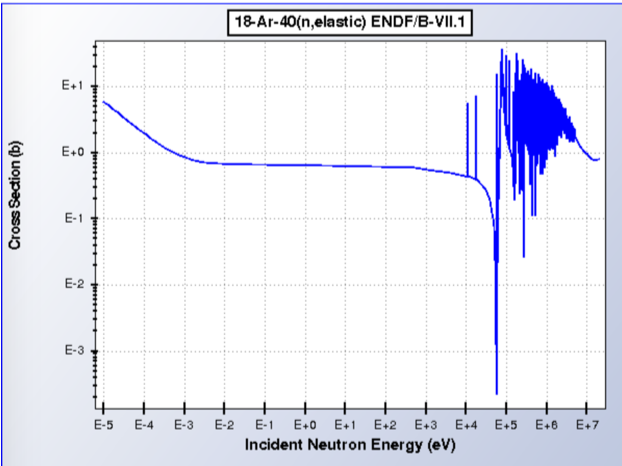
\includegraphics[width=0.4\linewidth]{Ar40xsec.png}
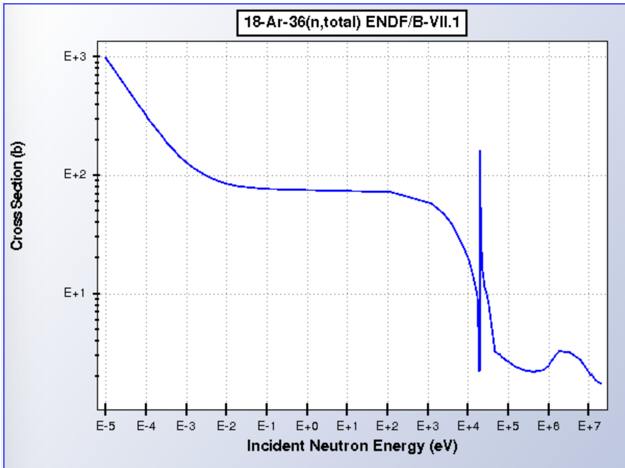
\includegraphics[width=0.4\linewidth]{Ar36xsec.png}
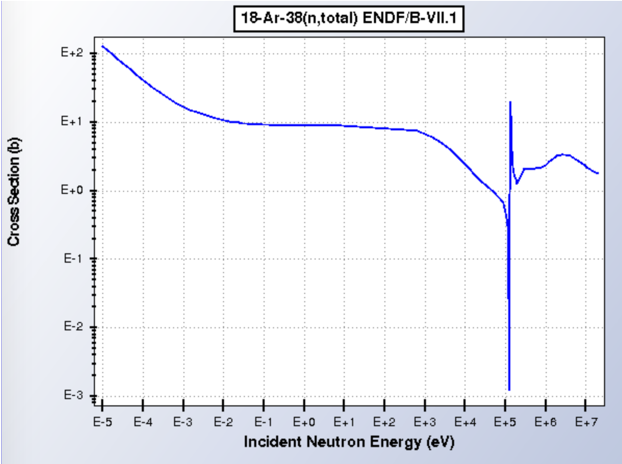
\includegraphics[width=0.4\linewidth]{Ar38xsec.png}
\end{dunefigure}
\fixme{NOTE: PUT IN PLOTS FOR ELASTIC}
Those that do scatter lose energy, leave the anti-resonance (where the scattering length is about \SI{70}{\cm}), quickly slow down and are captured. Each capture releases exactly the binding energy difference between \isotope{Ar}{40} and \isotope{Ar}{41}, about \SI{6.1}{\MeV} in the form of gamma rays.  As will be described below, by using a {\it DD Generator}\footnote{{\it DD} stands for "Deuterium-Deuterium" }, a triggered pulse of neutrons can be generated outside the TPC, then injected via a dedicated hole in the insulation into the \dword{lar}, where is spreads through the entire volume to produce "standard candle" \SI{6.1}{\MeV} energy depositions. Using this method, there would be no need for internal deployments, the calibration procedure would be quick (likely less than 30 minutes), and there is no need to manufacture short-lived isotopes at an external facility.

\begin{dunefigure}[h]{fig:Arxsec2}{Total scattering cross sections on 40-Ar in the range $10-200\; keV$~\cite{ref:ENDF}}
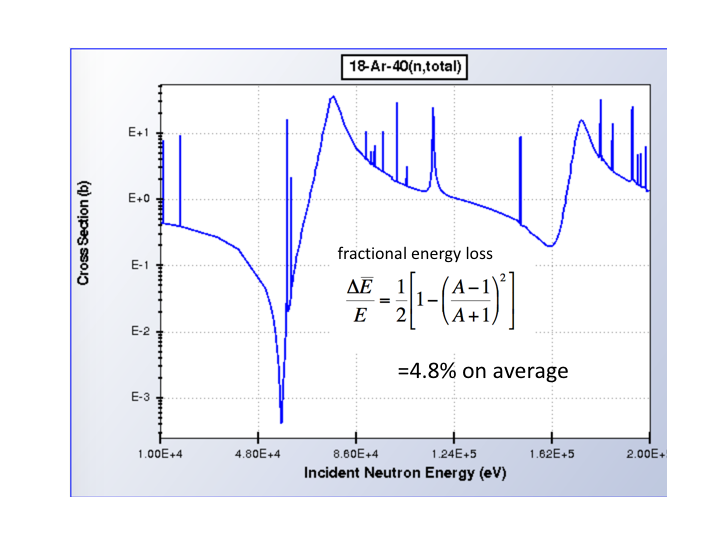
\includegraphics[width=0.75\linewidth]{Ar40Xsec2.png}
\end{dunefigure}

A relevant question is what fraction of neutrons slowing down from higher energy will fall into the anti-resonance. Figure~\ref{fig:Arxsec2} shows an expanded view of the total \isotope{Ar}{40} cross section in the range  \num{10} to \SI{200}{\keV}. Since the the average energy loss of a neutron elastically scattering off a \isotope{Ar}{40} nucleus is \num{4.8}\%, in the region of the anti-resonance the average energy loss per scatter is about \SI{3}{\keV}. Therefore, estimating the width of the anti-resonance to be about   \SI{10}{\keV}, a large fraction of the neutrons injected can be expected to fall into the cross section hole. Indeed, as will be shown in preliminary simulations, many neutrons scatter several times before escaping to lower energies to be captured. This simple phenomenon tends to scatter neutrons isotropically around the \dword{lar}.

\fixme{Mention Test at LANSCE and its role?}

%%%%%%%%%%%%%%%%%%%%%
\subsubsection{Design Considerations} 

%Figure~\ref{fig:PDLayout} shows a conceptual layout of the neutron injection system.

The fixed, shielded DD generator would \fixme{would go?} above a feedthrough in the hydrogenous insulation. Pulsed\footnote{The pulse width is \SI{100}{\micro\s}, but it is possible to reduce this by simply shortening the \dword{hv} pulse that sustains the reaction.}, commercially available DD generators exist and are cost competitive. Between the generator and the cryostat, \fixme{what would?} would include layers of water or plastic and intermediate fillers for sufficient degradation of the neutron energy.  Initial simulations indicate that a single neutron injection point would illuminate %all of ProtoDUNE's volume.
the entire volume of one of the \dword{protodune} detectors.

%{\it Additional details provided by  Bob. Add more here.}
%%%%%%%%%%%%%%%%%%%%%
\subsubsection{Remaining Studies}

The remaining studies for the TDR for the external neutron source are:
\begin{itemize}
\item ?? \fixme{Feedthrough collision? Where are we putting this and aren't the rest spoken for? Can we place and remove it with other radioactive sources? }
\item Assessment of the full design, including degrader materials and shielding.
\item Assessment of sufficient space and mounting (weight) considerations above the cryostat considering shielding for the neutron generator. 
\end{itemize}

\fixme{need to add some here }


%%%%%%%%%%%%%%%%%%%%%%%%%%%%%%%%%%%%%%%%%%%%%%%%%%%%%%%%%%%%%%%%%%%%%%%%%%%%%%%%%%%%%%%

Sample figure (Figure~\ref{fig:figure-label}):

\begin{dunefigure}[optional caption for LoF]{fig:figure-label}
{required full caption (Credit: xyz)}
%\includegraphics[width=0.8\textwidth]{image-filename}
\end{dunefigure}

Sample table (Table~\ref{tab:table-label}):

\begin{dunetable}
[optional caption for LoT]
{p{0.8\textwidth}}
{tab:table-label}
{required full caption}   
xyz  \\ \toprowrule
  \\ \colhline
   \\ \colhline
 ...\\ 
\end{dunetable}
